\documentclass[letterpaper,12pt]{scrartcl}
\usepackage{epsfig,latexsym,amsmath,amssymb,epic,eepic,psfrag,subfigure,float,euscript,array}
\usepackage[latin1]{inputenc}
\usepackage[margin=24mm]{geometry}
\usepackage{enumitem}
\usepackage{tikz,pgf,pgfplots}
\usepgfplotslibrary{fillbetween}
\usetikzlibrary{decorations, arrows}

\usepackage[amssymb]{SIunits}

\newenvironment{exercise}[1][Uppgift]{\begin{trivlist} \item[\hskip
    \labelsep {\stepcounter{exerctr}\bfseries #1
      \arabic{exerctr}}]}{\end{trivlist}\vspace{10mm}}

\newcounter{exerctr}
\newcounter{abcctr}[exerctr]

\newcommand{\abc}{\noindent\vspace{1mm}\\ {\bf
    \stepcounter{abcctr}(\alph{abcctr})\ }}
\newcommand{\bbm}{\begin{bmatrix}}
\newcommand{\ebm}{\end{bmatrix}}
\newcommand{\point}[1]{\hfill {\bf (#1p)}\\ \vspace{-5mm}}
\newcommand{\ctrb}{\EuScript{S}}
\newcommand{\Lap}{\mathcal{L}}
\newcommand{\obsv}{\EuScript{O}}
\newcommand{\realdel}{\text{Re}}
\newcommand{\imagdel}{\text{Im}}
\newcommand{\bC}{\mathbb{C}}
\newcommand{\bR}{\mathbb{R}}
\newcommand{\bmpv}{\begin{minipage}[t]}
\newcommand{\bmps}{\begin{minipage}[t]{45mm}}
\newcommand{\bmpm}{\begin{minipage}[t]{90mm}}
\newcommand{\bmpl}{\begin{minipage}[t]{\textwidth}}
\newcommand{\emp}{\end{minipage}}
\newcommand{\mexp}[1]{\ensuremath{\mathrm{e}^{#1}}}
\newcommand*{\laplaceinv}[1]{\ensuremath{\mathcal{L}^{-1} \left\{#1\right\}}}
\newcommand*{\ztrf}[1]{\ensuremath{\mathcal{Z} \left\{#1\right\}}}
\newcommand*{\shift}{\ensuremath{\operatorname{q}}}
\newcommand*{\diff}{\ensuremath{\operatorname{p}}}


\newcommand{\AxisRotator}[1][rotate=0]{%
    \tikz [x=0.2cm,y=0.60cm,line width=.1ex,-stealth,#1] \draw (0,0) arc (-150:150:1 and 1);%
}

\addtolength{\topmargin}{-8mm}
%\textheight 22.5cm
%\oddsidemargin 1.3cm
%\evensidemargin 1.3cm

\makeatletter
\newcommand*{\rom}[1]{\expandafter\@slowromancap\romannumeral #1@}
\makeatother

\newcommand*\circled[1]{\tikz[baseline=(char.base)]{
            \node[shape=circle,draw,inner sep=2pt] (char) {#1};}}


\title{Computerized Control partial exam 2 (15\%)}
\author{Kjartan Halvorsen}
\date{}

\begin{document}

\maketitle


\begin{description}
\item[Time] April 3 17:35-18.55
\item[Place] 5105
\item[Permitted aids] The single colored page with your own notes, table of Laplace transforms, calculator
\end{description}

All answers should be readable and well motivated (if nothing else is written). Solutions/motivations should be written on the provided spaces in this exam. Use the last page if more space is needed.

\begin{center}
{\Large Good luck!} \\
\end{center}

\noindent
\fbox{
\bmpl
{\bf Matricula and name:}\\
\vspace*{14mm}
\emp}


%\clearpage

%-----------------------------------------------------------------

\subsection*{Problem 1}
% PI controller, forward approximation

The euler forward approximation of a derivative is 
\[ \frac{d}{dt} f(t) \approx \frac{f(t+h)-f(t)}{h}, \]
which can be written using the derivative operator $\diff = \frac{d}{dt}$ and the shift operator $\shift$ as 
\[ \diff f \approx \frac{\shift - 1}{h} f. \]


\subsubsection*{(a)}
Use the forward approximation to find a discrete approximation $F_d(z)$ of the PI-controller
\[ F(s) = K(1 + \frac{1}{T_is}). \]

\noindent
\fbox{
\bmpl
{\bf Calculations and answer:}\\
\vspace*{64mm}
\emp}

\subsubsection*{(b)}
The block diagram below shows the discrete-time controller.
\begin{center}
  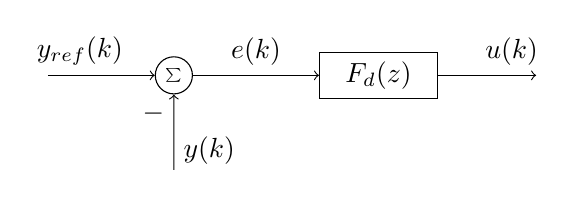
\begin{tikzpicture}[scale = 0.8, node distance=22mm, block/.style={rectangle, draw, minimum width=15mm}, sumnode/.style={circle, draw, inner sep=2pt}]
    
    \node[coordinate] (input) {};
     \node[sumnode, right of=input, node distance=16mm] (sum) {\tiny $\sum$};
     \node[block, right of=sum, node distance=26mm] (controller) {$F_d(z)$};
     \node[coordinate, right of=controller, node distance=20mm] (output) {};
     \node[coordinate, below of=sum, node distance=12mm] (feedback) {};

     \draw[->] (input) -- node[above, pos=0.3] {$y_{ref}(k)$} (sum);
     \draw[->] (sum) -- node[above] {$e(k)$} (controller);
     \draw[->] (controller) -- node[above, near end] {$u(k)$} (output);
     \draw[->] (feedback) -- node[right, near start] {$y(k)$} node [left, near end] {$-$} (sum);
   \end{tikzpicture}
   \end{center}
Write the controller as a \emph{difference equation} using $F_d(z)$ determined in (a).

\noindent
\fbox{
\bmpl
{\bf Calculations and answer:}\\
\vspace*{64mm}
\emp}


\subsection*{Problem 2}

The magnetic levitation (maglev) system below is an example of an unstable system. 
\begin{center}
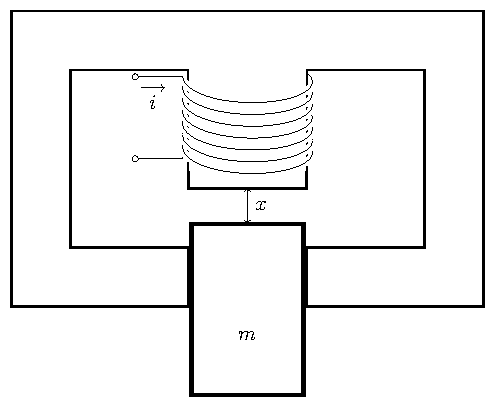
\includegraphics[width=0.4\linewidth]{../../../MR2004/figures/magnetic-suspension}
\end{center}
Ignoring friction in the system, a linearized model is given by the state space system
\begin{equation}
\begin{aligned}
  \dot{x}(t) &= \bbm 0 & 1\\ \omega^2 & 0 \ebm x(t) + \bbm 0\\1 \ebm u(t)\\
  y(t) &= \bbm 1 & 0 \ebm x(t),
\end{aligned}
\label{eq:maglevcont}
\end{equation}
with poles in $s = \pm \omega$. The input signal $u(t)$ is a deviation in the current $i(t)=i_0-u(t)$ applied to the windings, the state variable $x_1(t)$ is a deviation in the position of the suspension mass $z(t) = z_0 + x_1(t)$, and the state variable $x_2(t)$ is the velocity of the mass. The tuple ($i_0$, $z_0$, $\dot{z}=0$) forms an operating point, for which the system is in (unstable) equilibrium. 

Discretizing the system using zero-order-hold with $\omega=1$ and $\omega h = 0.2$  gives the discrete-time state space system
\begin{equation}
\begin{aligned}
  x(k+1) &= \underbrace{\bbm 1.02 & 0.20\\0.20 & 1.02 \ebm}_{\Phi} x(k) + \underbrace{\bbm 0.02\\0.20 \ebm}_{\Gamma} u(k)\\[2mm]
  y(t) &= \bbm 1 & 0 \ebm x(k).
\end{aligned}
\label{eq:maglev}
\end{equation}

\subsubsection*{(a)}

Determine the poles of the discrete-time open-loop system.

\noindent
\fbox{
\bmpl
{\bf Calculations and answer:}\\
\vspace*{64mm}
\emp}


\subsubsection*{(b)}

Assume that the state vector $x(k)$ must be estimated using an observer. Determine an observer gain vector $K$ such that the observer has poles in the origin.

\noindent
\fbox{
\bmpl
{\bf Calculations and answer:}\\
\vspace*{114mm}
\emp}
 
\subsection*{Problem 3}
A discrete-time controller with sampling period $h=0.2$ has been designed for the maglev system, according to the closed-loop block diagram in figure \ref{fig:block}. 
\begin{figure}[!h]
\begin{center}
  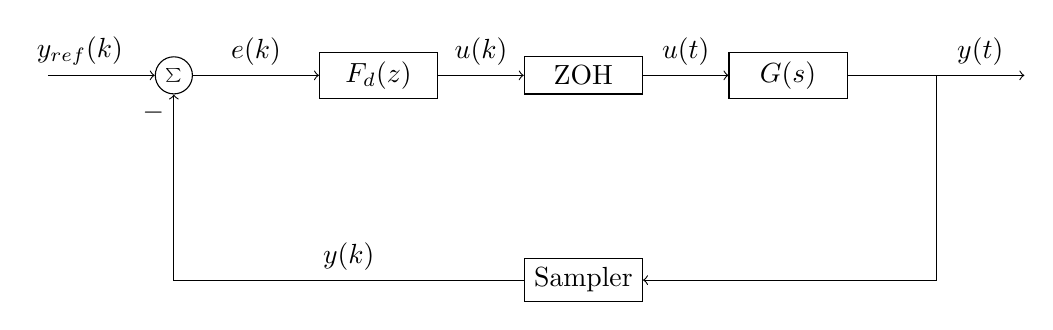
\begin{tikzpicture}[scale = 0.8, node distance=22mm, block/.style={rectangle, draw, minimum width=15mm}, sumnode/.style={circle, draw, inner sep=2pt}]
    
    \node[coordinate] (input) {};
     \node[sumnode, right of=input, node distance=16mm] (sum) {\tiny $\sum$};
     \node[block, right of=sum, node distance=26mm] (controller) {$F_d(z)$};
     \node[block, right of=controller, node distance=26mm] (zoh) {ZOH};
     \node[block, below of=zoh, node distance=26mm] (sampler) {Sampler};
     \node[block, right of=zoh, node distance=26mm] (plant) {$G(s)$};
     \node[coordinate, right of=plant, node distance=30mm] (output) {};

     \draw[->] (input) -- node[above, pos=0.3] {$y_{ref}(k)$} (sum);
     \draw[->] (sum) -- node[above] {$e(k)$} (controller);
     \draw[->] (controller) -- node[above] {$u(k)$} (zoh);
     \draw[->] (zoh) -- node[above] {$u(t)$} (plant);
     \draw[->] (plant) -- node[coordinate] (measure) {} node[above, near end] {$y(t)$} (output);
     \draw[->] (measure) |- (sampler);
     \draw[->] (sampler) -| node[above, near start] {$y(k)$} node [left, pos=0.95] {$-$} (sum);
   \end{tikzpicture}
   \end{center}
\caption{Discrete-time feedback control of the maglev system.}
\label{fig:block}
\end{figure}

Let $G_o(z)$ denote the loop gain (gain from $e(k)$ to $y(k)$) of the system, with bode diagram given in figure \ref{fig:loopgainbode}.

\begin{figure}[!h]
\begin{center}
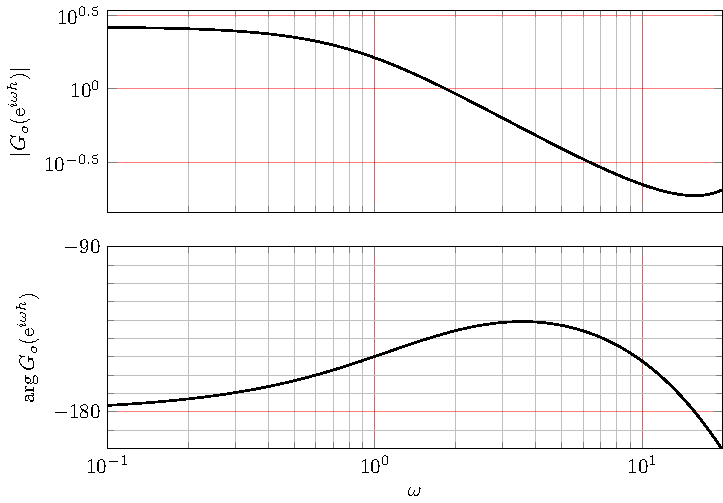
\includegraphics[width=0.9\linewidth]{../../figures/maglev_ss_loopgain_bode}
\end{center}
\caption{Bode diagram of the loop gain for the discrete-time control system in figure \ref{fig:block}.}
\label{fig:loopgainbode}
\end{figure}

\subsubsection*{(a)}
Determine the cross-over frequency and phase margin of the system.

\noindent
\fbox{
\bmpl
{\bf Answer:}\\
\vspace*{54mm}
\emp}



\subsubsection*{(b)}
In the design of the controller in the feedback system of figure \ref{fig:block} it was assumed that an anti-aliasing filter was not needed. However, later it was found that it was indeed necessary to filter the noise in the measured output signal $y(t)$. The modified control system is shown in figure \ref{fig:block-aa}. 
\begin{figure}[!h]
\begin{center}
  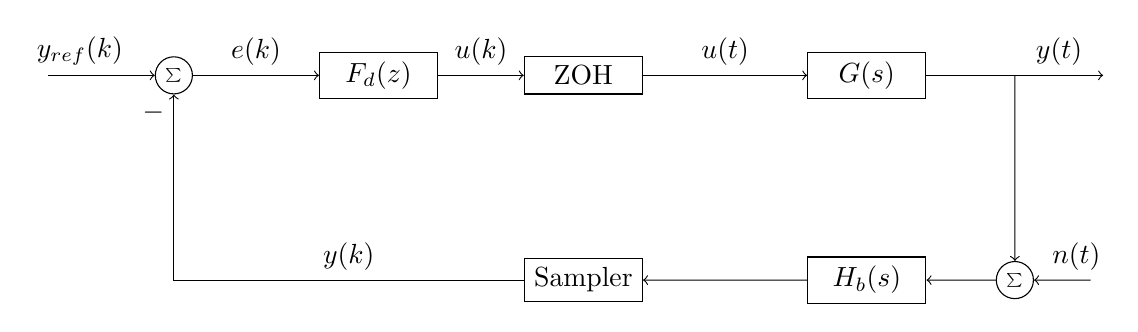
\begin{tikzpicture}[scale = 0.8, node distance=22mm, block/.style={rectangle, draw, minimum width=15mm}, sumnode/.style={circle, draw, inner sep=2pt}]
    
    \node[coordinate] (input) {};
     \node[sumnode, right of=input, node distance=16mm] (sum) {\tiny $\sum$};
     \node[block, right of=sum, node distance=26mm] (controller) {$F_d(z)$};
     \node[block, right of=controller, node distance=26mm] (zoh) {ZOH};
     \node[block, below of=zoh, node distance=26mm] (sampler) {Sampler};
     \node[block, right of=zoh, node distance=36mm] (plant) {$G(s)$};
     \node[block, below of=plant, node distance=26mm] (aa) {$H_b(s)$};
     \node[coordinate, right of=plant, node distance=30mm] (output) {};

     \draw[->] (input) -- node[above, pos=0.3] {$y_{ref}(k)$} (sum);
     \draw[->] (sum) -- node[above] {$e(k)$} (controller);
     \draw[->] (controller) -- node[above] {$u(k)$} (zoh);
     \draw[->] (zoh) -- node[above] {$u(t)$} (plant);
     \draw[->] (plant) -- node[coordinate] (measure) {} node[above, near end] {$y(t)$} (output);

     \node[sumnode, below of=measure, node distance=26mm] (sumnoise) {\tiny $\sum$};
     \draw[->] (measure) -- (sumnoise);
     \draw[->] (sumnoise) -- (aa);
     \draw[->] (sumnoise) ++(12mm,0) -- node[above, near start] {$n(t)$} (sumnoise);
     \draw[->] (aa) -- (sampler);
     \draw[->] (sampler) -| node[above, near start] {$y(k)$} node [left, pos=0.95] {$-$} (sum);
   \end{tikzpicture}
   \end{center}
\caption{Discrete-time feedback control of the maglev system with anti-aliasing filter.}
\label{fig:block-aa}
\end{figure}

The anti-aliasing filter $H_b(s)$ is a second-order Bessel filter with Bode diagram given below. 
\begin{center}
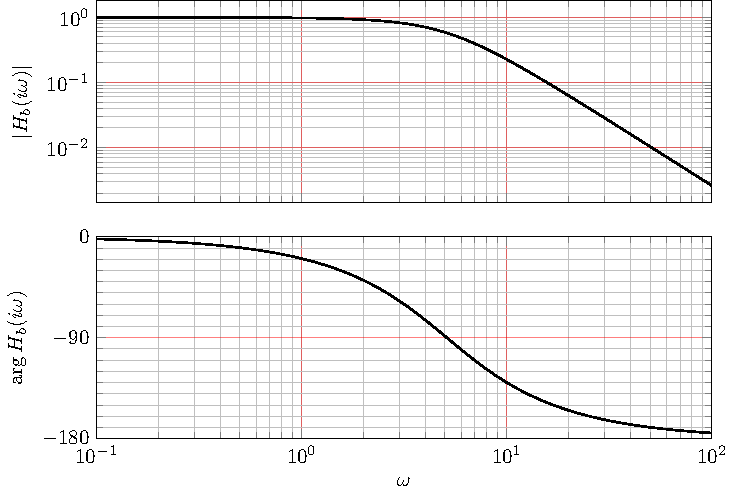
\includegraphics[width=0.8\linewidth]{../../figures/maglev_bessel_aa_bode}
\end{center}
What is the phase margin of the control system \textbf{with} anti-aliasing filter? How would you \textbf{describe} such a closed-loop system?

\noindent
\fbox{
\bmpl
{\bf Calculations and answer:}\\
\vspace*{104mm}
\emp}


\cleardoublepage

\section*{Solutions}

\subsection*{Problem 1}

\subsubsection*{(a)}
The forward approximation becomes
\[ F_d(z) = F(s)|_{s = \frac{z-1}{h}} = K(1 + \frac{1}{T_i\frac{z-1}{h}}) = K( 1 + \frac{h}{T_i(z-1)}). \]

\subsubsection*{(b)}
The controller is
\[ U(z) = F_d(z)E(z), \]
which using the pulse transfer operator can be written
\[ u(kh) = K(1 + \frac{h}{T_i(\shift-1)}) e(kh) = K \frac{\shift-1 + \frac{h}{T_i}}{\shift-1} e(kh)\]
\[ (\shift -1) u(kh) = K(\shift -1+\frac{h}{T_i}) e(kh)\]
\[ u(kh+h) - u(kh) = K\big(e(kh+h) - (1-\frac{h}{T_i})e(kh)\big)\]
\[ u(kh+h) = u(kh) + K\big(e(kh+h) - (1-\frac{h}{T_i})e(kh)\big)\]

\subsection*{Problem 2}

\subsubsection*{(a)}
The poles are given by the eigenvalues of the $\Phi$ matrix, which in turns are the solutions to the characteristic equation \( \det (zI - \Phi) = 0\). With
\[ \Phi = \bbm 1.02 & 0.20\\0.20 & 1.02 \ebm, \]
we get
\[ \det \bbm z - 1.02 & -0.20\\ -0.20 & z-1.02 \ebm = (z-1.02)^2 - 0.2^2 = z^2 -2.04z + 1.02^2 - 0.2^2.\]
with solutions
\[ z = 1.02 \pm \frac{1}{2}\sqrt{(-2.04)^2 - 4(1.02^2 - 0.2^2)} = \begin{cases} 1.22\\0.82 \end{cases}. \]
Evidently one of the poles are outside the unit circle.

  
\subsubsection*{(b)}
The dynamics of the observer is given by
\[\hat{x}(k+1) = \big(\Phi - KC\big)\hat{x}(k) + \Gamma u(k) + Ky(k),\] where
\[ KC = \bbm k_1\\k_2 \ebm \bbm 1 & 0 \ebm = \bbm k_1 & 0\\k_2 & 0\ebm.\]
The characteristic polynomial becomes
\begin{equation*}
\begin{aligned}
\det \big( zI - (\Phi-KC)\big) &= \det \left( \bbm z & 0 \\ 0 & z \ebm - \bbm 1.02-k_1 & -0.2\\0.2-k_2 & 1.02\ebm\right)\\
&= \det \bbm z-1.02+k_1 & -0.2\\-0.2+k_2 & z-1.02\ebm = (z-1.02+k_1)(z-1.02) + 0.2(-0.2+k_2)\\
&= z^2 + (-2.04 + k_1)z - 1.02(k_1-1.02) - 0.2^2 + 0.2k_2 = z^2 + (k_1-2.04)z - 1.02k_1 + 0.2k_2 + 1.02^2 - 0.2^2.
\end{aligned} 
\end{equation*}
Comparing with the desired characteristic polynomial (poles in the origin) $z^2$, we get the equations
\begin{align*}
k_1 - 2.04 &= 0\\
- 1.02k_1 + 0.2k_2 + 1.02^2 - 0.2^2 &= 0
\end{align*}
with solution
\[ K = \bbm k_1\\k_2 \ebm = \bbm 2.04\\5.40 \ebm.\]

\subsection*{Problem 3}

\subsubsection*{(a)}
\begin{center}
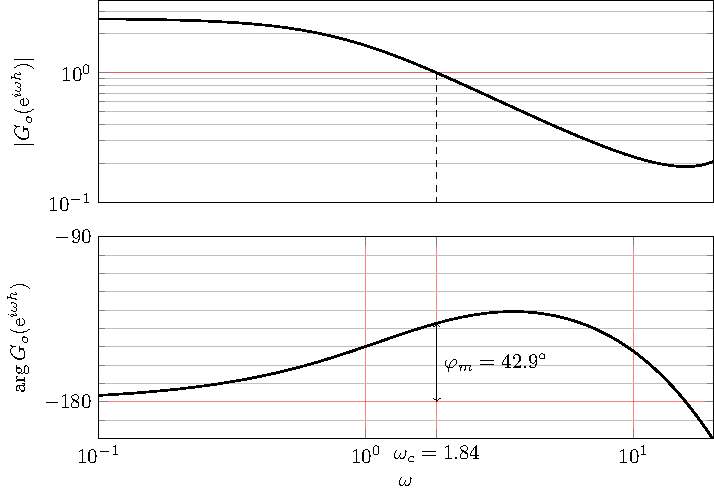
\includegraphics[width=0.9\linewidth]{../../figures/maglev_ss_loopgain_bode_sol}
\end{center}

\subsubsection*{(b)}
At the cross-over frequency the bessel filter has a phase of about $-36^\circ$. 
\begin{center}
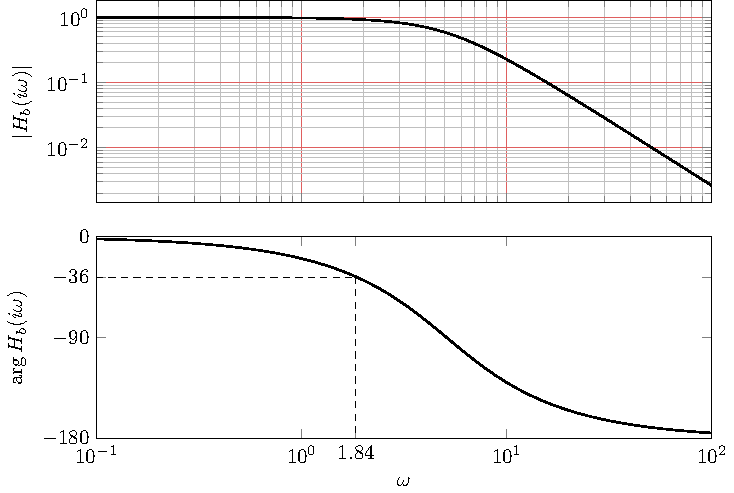
\includegraphics[width=0.8\linewidth]{../../figures/maglev_bessel_aa_bode_sol}
\end{center}
This means that the phase margin for the system \textbf{with} anti-aliasing filter becomes 
\[ \varphi_m = 42.9 - 36 = 6.9^\circ.\] A closed-loop system with this little phase margin will have a large resonance peak and an oscillatory response. 


\end{document}
